\section{ Basic multi-photon systems and their curves }
Various exposure curves can be implemented in 
hypothetical normalized systems as shown here.
This topic includes a comparison of systems with real and
virtual intermediate states which has been discussed
in more detail in contemporary works looking at
multiphoton system measurement
\cite{Masthay_Beach_Eckerle_Photochemical_characterization_rate_2024}
 for example.

This analysis relates to the idea expressed in 
Fukuda in 2025 \cite{Fukuda_Statistics_exposed_2025}
that part of the problem with EUV vs DUV 
is in the resist dealing with image contrast.
Other issues are moved from developer chemistry to 
earlier photocarrier involved reactions although
the author does go on to explain how effecitvely
multi-photons are required anyway for development. 

A simple n-photon system can repdouce the curves from 
the prior section but more complicated or modified
real systems may be more difficult to analyze. 
In the following a constant light flux, $\phi$,
illuminates a variety of chemical species denoted
by capital letters. Arbitrary constants are included
only to illustrate specific issues. While encountered in 
real implementations, they may obscure the initial dynamics.
Note too that some cases such as very high photon number may
not be realizable with any practical or known system but illustrate
potential benefits if such a system could be created. 
 
\subsection{ Cascade or Ladder  }
This is the "pure" multi-photon system where a developer
responds to some species which requires n photons to synthesize.

\begin{comment} 
\cee{ 2Cu^{++}  + 4I^-  -> 2CuI +  I_2}
Once Cu(I) is formed, it can undergo underirable reacions.
\cite{SAMUNI_ARONOVITCH_GODINGER_cytotoxicity_1983}
\cee{ Cu^+ + H_2O_2  -> Cu^{++} +  OH^- +  OH }
disproportionation,
\cee{ 2Cu^+ (sq)  -> Cu^{++}(aq) +  Cu(s) }
\end{comment} 

Consider a cascade or ladder or serial processes such that
\cee{  X_i + h$\nu$ -> X_{i+1} }

for i=0 to i=n-1. The rate equations then are 
% moved to doc need to add to include file 
%\newcommand{\mjmdt}[1]{\frac{d#1}{dt}} \newcommand{\mjmdtt}[1]{\frac{d^2#1}{dt^2}} \newcommand{\mjmdphi}[1]{\frac{d#1}{d\phi}}



\mjmeqn{ \mjmdt{X_{i}} = c\phi X_{i-1} - c\phi X_{i}}  
and for i==0,
\mjmeqn{ X_0(t)=X_0(0)exp(-c\phi t) }  
and for i==n,
\mjmeqn{ \mjmdt{X_{n}} = c\phi X_{i-1} }  

Successively integrating gives,
\mjmeqn{ X_{i+1}(t)=X_i(0)\frac{(c\phi t ) ^ (i+1)}{(i+1)!}exp(-c\phi t) }
 except at the ends points. $X_0$ was already given and
$X_n$ lacking the photoconversion to another species gives


\mjmeqn{ X_{n} = X_0(0)( 1- \exp(-c\phi t) \sum_0^{n-1} \frac{(c\phi t)^i}{i!}  ) \label{eqn:multip} }

\mjmeqn{ X_{n}/X_0(0) = 1- \exp(-c\phi t) \sum_0^{n-1} \frac{(c\phi t)^i}{i!}   }

  
which is exactly the  ( complement of the  ) Poisson probability of exposure
\mjmrefeqn{basicsum} with $<n> = c\phi t $   and $n_t=n-1$
 the most number of photons that fail to create a developable feature. 


\subsection{ Cascade or Ladder with Finite Lifetime States  }

The above specialized case reproducted the Poisson probability of
failure and is a good limiting case for further work. 
Before getting to the system normally called multi-photon in which
all photons are absorbed simultaneously, it may be usful to look
at the case of a finite lifetime intermediate state or a leaky
integrator of photon flux. 

The general system is, 

\begin{figure}[htb]
\centering

\cee{  X_0 + h$\nu$ -> X_1 }

\cee{  X_{i-1} + h$\nu$ -> X_i }

for i not equal zero or n,

\cee{  X_i ->[k] X_{i-1} }

\mjmeqn{\mjmdt{X_i}=-\phi X_i+\phi X_{i-1} + k X_{i+1}-k X_i }

otherwise with no decay from terminal state,

\mjmeqn{\mjmdt{X_n}=\phi X_{n-1} }
\mjmeqn{\mjmdt{X_{n-1}}=-\phi X_{n-1}+\phi X_{n-2} -k X_n-1 }

\mjmeqn{\mjmdt{X_0}=-\phi X_0+ k X_{1} }


\caption{ Leaking integrators with loss finite lifetime states but stable terminal state . }
\label{fig:leakyn} 
\end{figure}


%\mjmpicture{plotleak.png}{ Some exposure curves demonstrating less confusion with the loss terms. The y-axis is P of developing while the X-axis is photon flux with exposure time adjusted to get overlapping curves.    }{plotleak}

{
\begin{figure}[H]
{ 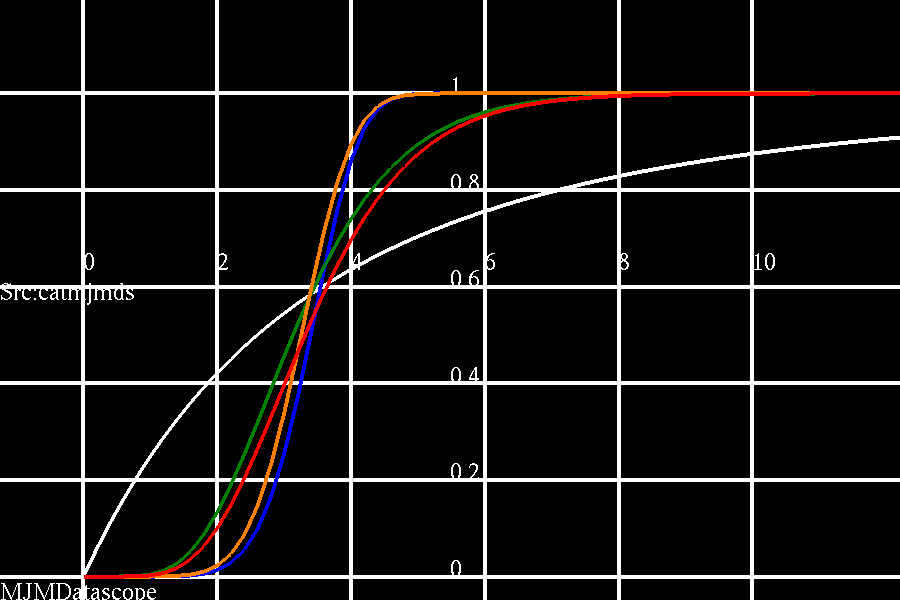
\includegraphics[height=3in,width=4in]{keep/plotleak.png} }
\begin{tabular}{|r|r|r|r|r|r|r|}
\hline
\multicolumn{7}{|c|}{Leaky Response Curve Parameters }\\
\hline
color & n-species &k & exp time & phi-10 & phi-50 &phi-90 \\
\hline
white & 2 &- & .3 & 0.358753 &  2.59927 &  11.5451 \\
green & 10 &0 & 2.75 &  1.85584 &  3.13446 &  5.05911 \\
red & 10 &.5 &  3 &   2.00123  &   3.31509 &  5.24203 \\
orange & 10 &5 &  50 &  2.4503 &  3.25675 &  4.02285 \\
blue  & 10 & 6 &  100 & 2.6079  &    3.39818 &  4.11833 \\
\hline
\end{tabular}
\caption{ Some exposure curves demonstrating less confusion with the loss terms. The y-axis is P of developing while the X-axis is photon flux with exposure time adjusted to get overlapping curves. The exposure time ratio is 333 between 1 photon and the very lossy case. Note that the values here for illustration and may not reflect typial realizable systems of interest  ./plotleak  }
\label{fig:plotleakt}
\end{figure} 
} % mjmpicture
 





\begin{comment}
\begin{table}[H] \centering
\begin{tabular}{|r|r|r|r|r|r|r|}
\hline
\multicolumn{7}{|c|}{Leaky Response Curve Parameters }\\
\hline
color & n-species &k & exp time & phi-10 & phi-50 &phi-90 \\
\hline
white & 2 &- & .3 & 0.358753 &  2.59927 &  11.5451 \\
green & 10 &0 & 2.75 &  1.85584 &  3.13446 &  5.05911 \\
red & 10 &.5 &  3 &   2.00123  &   3.31509 &  5.24203 \\
orange & 10 &5 &  50 &  2.4503 &  3.25675 &  4.02285 \\
blue  & 10 & 6 &  100 & 2.6079  &    3.39818 p&  4.11833 \\
\hline
\end{tabular}

\caption{}
%\label{}
\end{table}
\end{comment}




If this seems familiar its redundant with 
preceding section in mjm\_euv\_multi.tex.
However, the terms are grouped differently to show tri-diagonal
structure and detail the corner cases for small n.
I wrote "mjm\_math" to do a few polynomial manipulations
although it could probably be done in a variety of existing
things like mathematica or sympy. 

\begin{figure}[htb]
\centering

\cee{  X_0 + h$\nu$ -> X_1 }

\cee{  X_{i-1} + h$\nu$ -> X_i }

for i not equal zero or n,

\cee{  X_i ->[k] X_{i-1} }

\mjmeqn{\mjmdt{X_i}=-\phi X_i+\phi X_{i-1} + k X_{i+1}-k X_i 
= \phi X_{i-1} -(\phi + k )  X_i + k X_{i+1} }

otherwise with no decay from terminal state,

\mjmeqn{\mjmdt{X_n}=\phi X_{n-1} }
\mjmeqn{\mjmdt{X_{n-1}}=-(\phi+k) X_{n-1}+\phi X_{n-2}  }
\mjmeqn{\mjmdt{X_0}=-\phi X_0+ k X_{1} }


\caption{ With loss finite lifetime states but stable terminal state . }
\label{fig:leakynrepeat}
\end{figure}

\mjmtol{

wtf n=2,
%\mjmeqn{\mjmdt{X_2}=\phi X_{1} }
%\mjmeqn{\mjmdt{X_{1}}=-(\phi+k) X_{1}+\phi X_{0}  }
%\mjmeqn{\mjmdt{X_0}=-\phi X_0+ k X_{1} }


\mjmeqn{\mjmdtn{2}{X_2}=\phi \mjmdt{X_{1}} }
\mjmeqn{\mjmdtn{2}{X_2}=\left( -(\phi+k)\phi X_{1}+\phi^2 X_{0}   \right) } 
\mjmeqn{\mjmdtn{2}{X_2}=\left( -(\phi+k)\mjmdt{X_{2}}+\phi^2 X_{0}   \right) } 
\mjmeqn{\mjmdtn{2}{X_2}+(\phi+k)\mjmdt{X_{2}}= \phi^2 X_{0}    } 
\mjmeqn{\mjmdtn{3}{X_2}+(\phi+k)\mjmdtn{2}{X_{2}}= \phi^2 \mjmdt{X_{0}  }  } 
\mjmeqn{\mjmdtn{3}{X_2}+(\phi+k)\mjmdtn{2}{X_{2}}
= \phi^2 \left( -\phi X_0+ k X_{1} \right)  }  

\mjmeqn{\mjmdtn{3}{X_2}+(\phi+k)\mjmdtn{2}{X_{2}}
= -\phi^3 X_0+ k\phi \mjmdt{ X_{2} }  }  

\mjmeqn{\mjmdtn{3}{X_2}+(\phi+k)\mjmdtn{2}{X_{2}}
- k\phi \mjmdt{X_{2}}  = -\phi^3 X_0 }  

\mjmeqn{\mjmdtn{3}{X_2}+(\phi+k)\mjmdtn{2}{X_{2}}
- k\phi \mjmdt{X_{2}}  = 
-\phi  \left( \mjmdtn{2}{X_2}+(\phi+k)\mjmdt{X_{2}} \right)
}  
\mjmeqn{\mjmdtn{3}{X_2}+(2*\phi+k)\mjmdtn{2}{X_{2}}
+\phi^2 \mjmdt{X_{2}}  = 0
}  
\mjmeqn{ r(r^2+(2\phi+k)r+\phi^2) =0 }

\mjmeqn{ b^2=4\phi^2+k^2+4k\phi  }
\mjmeqn{ b^2-4ac=k^2+4k\phi  }
\mjmeqn{ r=-\phi-\frac{k}{2} \pm \sqrt{k(k+4\phi)}   }

} % mjtol 


\mjmtol{

 n=3,
\mjmeqn{\mjmdt{X_3}=\phi X_{2} }
\mjmeqn{\mjmdt{X_{2}}=-(\phi+k) X_{2}+\phi X_{1}  }
\mjmeqn{\mjmdt{X_{1}}=-(\phi+k) X_{1}+\phi X_{0}-k X_{2}  }
\mjmeqn{\mjmdt{X_0}=-\phi X_0+ k X_{1} }


\mjmeqn{\mjmdtn{2}{X_3}=\phi \mjmdt{X_{2}} }
\mjmeqn{\mjmdtn{2}{X_3}=\left( -(\phi+k)\phi X_{2}+\phi^2 X_{1}   \right) } 
\mjmeqn{\mjmdtn{2}{X_2}=\left( -(\phi+k)\mjmdt{X_{3}}+\phi^2 X_{1}   \right) } 
\mjmeqn{\mjmdtn{2}{X_3}+(\phi+k)\mjmdt{X_{3}}= \phi^2 X_{1}    } 


\mjmeqn{\mjmdtn{3}{X_3}+(\phi+k)\mjmdtn{2}{X_{3}}= \phi^2 \mjmdt{X_{1}}    } 

\mjmeqn{\mjmdtn{3}{X_3}+(\phi+k)\mjmdtn{2}{X_{3}}= \phi^2 
%\mjmdt{X_{1}}    
\left( -(\phi+k) X_{1}+\phi X_{0}-k X_{2}  \right)
} 

\mjmeqn{\mjmdtn{3}{X_3}+(\phi+k)\mjmdtn{2}{X_{3}}=  
%-\phi^2(\phi+k) X_{1}
-(\phi+k)(\mjmdtn{2}{X_3}+(\phi+k)\mjmdt{X_{3}})  
+\phi^3 X_{0}
%-k\phi^2 X_{2}  
-k\phi \mjmdt{X_{3} } 
} 

\mjmeqn{\mjmdtn{3}{X_3}+2(\phi+k)\mjmdtn{2}{X_{3}}
+((\phi+k)^2+k\phi)\mjmdt{X_{3}})  
=  \phi^3 X_{0}
} 

%\mjmeqn{\mjmdt{X_0}=-\phi X_0+ k X_{1} }
\mjmeqn{\mjmdtn{4}{X_3}+2(\phi+k)\mjmdtn{3}{X_{3}}
+((\phi+k)^2+k\phi)\mjmdtn{2}{X_{3}})  
=   
 -\phi^4 X_0
+ k\phi^3 X_{1} 
} 



} % ssck n=3
\mjmtol{ n==3 part 2

repeat,

\mjmeqn{\mjmdtn{4}{X_3}+2(\phi+k)\mjmdtn{3}{X_{3}}
+((\phi+k)^2+k\phi)\mjmdtn{2}{X_{3}})  
=   
 -\phi^4 X_0
+ k\phi^3 X_{1} 
} 

use identities,
\mjmeqn{\mjmdtn{3}{X_3}+2(\phi+k)\mjmdtn{2}{X_{3}}
+((\phi+k)^2+k\phi)\mjmdt{X_{3}})  
=  \phi^3 X_{0}
} 
\mjmeqn{\mjmdtn{3}{X_3}+(\phi+k)\mjmdtn{2}{X_{3}}= \phi^2 \mjmdt{X_{1}}    } 
\mjmeqn{\mjmdtn{2}{X_3}+(\phi+k)\mjmdt{X_{3}}= \phi^2 X_{1}    } 

\mjmeqn{\mjmdtn{4}{X_3}+2(\phi+k)\mjmdtn{3}{X_{3}}
+((\phi+k)^2+k\phi)\mjmdtn{2}{X_{3}})  
=   
% -\phi^4 X_0
-\phi\mjmdtn{3}{X_3} -\phi 2(\phi+k)\mjmdtn{2}{X_{3}}
-\phi((\phi+k)^2+k\phi)\mjmdt{X_{3}})  
%+ k\phi^3 X_{1} 
+k\phi\mjmdtn{2}{X_3}+k\phi(\phi+k)\mjmdt{X_{3}} 
} 

\mjmeqn{\mjmdtn{4}{X_3}
+(3\phi+2k)\mjmdtn{3}{X_{3}}
+((\phi+k)^2+2k\phi+2\phi^2)\mjmdtn{2}{X_{3}}  
+\phi((\phi+k)^2-k*k)\mjmdt{X_{3}}  
=  0 
% -\phi^4 X_0
%+ k\phi^3 X_{1} 
} 


\mjmeqn{\mjmdtn{4}{X_3}
+(3\phi+2k)\mjmdtn{3}{X_{3}}
%+((\phi+k)^2+2k\phi+2\phi^2)\mjmdtn{2}{X_{3}}  
+(k^2+4k\phi +3\phi^2)\mjmdtn{2}{X_{3}}  
%+\phi((\phi+k)^2-k*k)\mjmdt{X_{3}}  
+(\phi^3+2k\phi^2 )\mjmdt{X_{3}}  
=  0 
% -\phi^4 X_0
%+ k\phi^3 X_{1} 
} 




} % n==3 part2




The characteristic equation then is,

\mjmeqn{\mjmdtn{2}{X_n}=\phi \mjmdt{X_{n-1}} }
\mjmeqn{\mjmdtn{2}{X_n}=
  \phi  \left( -(\phi+k) \mjmdt{X_{n-1}}+\phi \mjmdt{X_{n-2}}   \right) }

\mjmeqn{\mjmdtn{2}{X_n}=
  \phi  \left( -(\phi+k)\mjmdt{X_n}+\phi \mjmdt{X_{n-2}} \right) }

\mjmeqn{\mjmdtn{2}{X_n}=
   -(\phi+k)\phi\mjmdt{X_n}+\phi^2 \mjmdt{X_{n-2}}  }

\mjmeqn{\mjmdtn{2}{X_n}+ (\phi+k)\phi \mjmdt{X_n}
=\phi^2 \mjmdt{X_{n-2}}  }

For n=2, 
%\mjmeqn{\mjmdtn{2}{X_2}+ (\phi+k) \mjmdt{X_2} =\phi^2\left( -\phi X_0+ k X_{1} \right) =-\phi^3 X_0+ k\phi^2 \mjmdt{X_{2}} }
%\mjmeqn{\mjmdtn{2}{X_2}+ (\phi+k) \mjmdt{X_2} =\phi^2\left( -\phi X_0+ k X_{1} \right) =-\phi^3 X_0+ k \phi X_{1} }


\mjmeqn{\mjmdtn{2}{X_2}+ (\phi+k)\phi \mjmdt{X_2}
=\phi^2\left( -\phi X_0+ k X_{1} \right)
=-\phi^3 X_0+ k\phi \mjmdt{X_{2}} 
}


\mjmeqn{\mjmdtn{2}{X_2}+\phi^2\mjmdt{X_2} =-\phi^3 X_0 }

\mjmeqn{\mjmdtn{3}{X_2}+ \phi^2  \mjmdtn{2}{X_2} =-\phi^3 \mjmdt{X_0}
= \phi^4 X_0 - \phi^3 k X_1
 }
\mjmeqn{\mjmdtn{3}{X_2}+ \phi^2 \mjmdtn{2}{X_2} =-\phi^3 \mjmdt{X_0}
= 
% \phi^4 X_0 
- \phi \mjmdtn{2}{X_2} - \phi^3\mjmdt{X_2} 
- \phi^3 k X_1
 }

\mjmeqn{\mjmdtn{3}{X_2}+ (\phi^2+\phi ) \mjmdtn{2}{X_2} 
+ \phi^3 \mjmdt{X_2} 
=- \phi^3 k X_1 = -\phi^2 k \mjmdt{X_2}
 }

%%%%%%%%%%%%%%%%%%%%%%%%%%%%%%%%%%%%%%


\mjmeqn{\mjmdtn{3}{X_2}+ (\phi^2+\phi ) \mjmdtn{2}{X_2} 
+  ( \phi^3 +\phi^2 k) \mjmdt{X_2} =0 
 }


\mjmeqn{ r(r^2+r(\phi+\phi^2)+\phi^2(\phi+k) ) =0 }

\mjmeqn{ b^2=  \phi^2(1+2\phi+\phi^2)  }
\mjmeqn{ b^2-4ac=  \phi^2(1+2\phi+\phi^2)-4*\phi^2(\phi+k)   }



%\mjmeqn{\mjmdtn{3}{X_2}+ (\phi+k-k\phi ) \mjmdtn{2}{X_2} =-\phi^3 \mjmdt{X_0} =-\phi \left( \mjmdtn{2}{X_2}+ (\phi+k) \mjmdt{X_1} \right) }


%\mjmeqn{\mjmdtn{3}{X_2}+ (2*\phi+k-k\phi ) \mjmdtn{2}{X_2} =-  (\phi+k) \mjmdtn{2}{X_2} }










The silver halids
and probably other systems will have more paramter variation and
more physical effects making the equations more complicated. With computers
and numerical codes it may not seem worthwhile to explore these 
analytically but they are useful for early thinking about 
candidate photo systems. 

In a simple  2 photon process a light flux $\phi$ converts A into B
and a potentially different flux or different rate, $\psi$,  converts
B into C. B can also decay back to A. 

\begin{figure}[htb]
\centering

\cee{  A + h$\nu$ -> B }

\cee{  B + h$\nu_2$ -> C }

\cee{  B ->[k_1] A }

\mjmeqn{\mjmdt{A}=-\phi A + k_1 B }

\mjmeqn{\mjmdt{B}=\phi A - k_1 B - \psi B  }

\mjmeqn{\mjmdt{C}=\psi B  }

\caption{ With loss of unstable intermediate B   }
\label{fig:loss} 
\end{figure}

As before variables can be eliminated and a single higher order
linear equation can be solved. 

% showworkcomment
\mjmwork{characteristic eqn }{
\mjmeqn{\mjmdtt{A}=-\phi \mjmdt{A} + k_1 \mjmdt{B} }

\mjmeqn{\frac{1}{k_1}(\mjmdtt{A}+\phi \mjmdt{A}) = \mjmdt{B} }

\mjmeqn{\frac{1}{k_1}(\mjmdt{A}+\phi A )=  B }

\mjmeqn{\mjmdt{B}=\phi A - k_1 B - \psi B  = \phi A -(k_1 + \psi)B }


\mjmeqn{\frac{1}{k_1}(\mjmdtt{A}+\phi \mjmdt{A}) = \phi A - k_1 B - \psi B  = \phi A -(k_1 + \psi)( \frac{1}{k_1}(\mjmdt{A}+\phi A )) }
\mjmeqn{\frac{1}{k_1}(\mjmdtt{A}+\phi \mjmdt{A}) =  \phi A -(k_1 + \psi)( \frac{1}{k_1}(\mjmdt{A}+\phi A )) }

\mjmeqn{\frac{1}{k_1}\mjmdtt{A} +\frac{1}{k_1}\phi \mjmdt{A} =  (\phi-\frac{\psi\phi}{k_1} -\phi ) A -(k_1 + \psi)\frac{1}{k_1}\mjmdt{A}  }

\mjmeqn{\frac{1}{k_1}\mjmdtt{A} +(k_1 + \psi+\phi)\frac{1}{k_1}\mjmdt{A}  + \frac{\phi\psi}{k_1} A  = 0 }

\mjmeqn{\mjmdtt{A} +(k_1 + \psi+\phi)\mjmdt{A}  +\phi\psi   A  = 0 }

\mjmeqn{r = -\frac{(k_1 + \psi+\phi)}{2}  \pm \frac{1}{2}\sqrt{(k_1+\psi+\phi)^2 -4\phi\psi }  }


\mjmeqn{r = -\frac{(k_1 + \psi+\phi)}{2}  \pm \frac{1}{2}\sqrt{k_1^2+2k_1*(\phi+\psi) +(\psi+\phi)^2 -4\phi\psi }  }

\mjmeqn{r = -\frac{(k_1 + \psi+\phi)}{2}  \pm \frac{1}{2}\sqrt{k_1^2+2k_1*(\phi+\psi) +(\psi-\phi)^2  }  }

} % mjmwork
Its probably worth nothing that the earlier system had degenerate roots
and this one may approach that.  Consider two roots r and $(r+\delta)$
and pairs of  constants $A_x$ and $A_y$ defined below. 
In the limit of small $\delta t $ the exponential can be expanded
although for finite $\delta$ this will always grow with time.

% showworkcomment
\mjmwork{degenerate roots }{
\mjmeqn{ A= A_-e^{rt} + A_+e^{(r +\delta)t  } ;
\mjmdt{A} = A_-re^{rt} + A_+(r+\delta)e^{(r +\delta)t}}

\mjmeqn{ A(0)= A_- + A_+ ;  
\mjmdt{A}(0) = A_-r + A_+(r+\delta)=-\phi A(0)}

\mjmeqn{ rA(0) + A_+\delta = - \phi A(0) }
\mjmeqn{ (\phi + r)A(0) =- A_+\delta } 
Using "engineering ( aka gutter ) math" take limit as delta goes to zero,

\mjmeqn{ A= e^{rt}(A_z + A_d(1+\delta t))  } ;
change variables, 
} % degenerate roots 

The general solution can be written as, 
\mjmeqn{ A= e^{rt}(A_1 + A_2\delta t)  } ;
with 
\mjmeqn{ \mjmdt{A}= e^{rt}( A_2\delta+ rA_1+rA_2\delta t )  } ;
and its possible to solve for $A_2\delta$ product,
\mjmeqn{ A(0)= A_1 } ;
\mjmeqn{ \mjmdt{A}(0)= (  rA(0)+A_2\delta(1+0) )  } ;
\mjmeqn{ A_2\delta= \mjmdt{A}(0)- rA(0)  } ;
or   
\mjmeqn{ A= e^{rt}(A(0) + (\mjmdt{A}(0)-rA(0)) t)  } ;

In any case the discriminant is positive semidefinite and 
an osillatory response is not possible. 




\subsection{ Simultaneous Multi-photon Absorption  }

One point of this work is to use the multi-photon term 
for processes such as the above although in general usage for
EUV it seems to be specialized to simulateous absorption
of n-photons or proceeeding through virtual states. 
As shown in the previous section, the temporal correlation 
related to the leaky integration helps to sharpen the curve
and in fact the simultaneous curve does appear to have a
smaller zone of confusion than the long lived intemediate state
case for same number of required photons but of course it
wastes more. 

\begin{figure}[htb]
\centering

\cee{  A + nh$\nu$ -> B }


\mjmeqn{ \mjmdt{A} =   -A \phi^n }  
\mjmeqn{ \mjmdt{B} =   A \phi^n }  
\mjmeqn{A(t)=A(0)(exp(-\phi^n  t )) }

\mjmeqn{ \mjmdt{B} =   \phi^n A(0)(exp(-\phi^n  t )) }
\mjmeqn{ B(t) =   A(0)(1-exp(-\phi^n  t )) }

\mjmeqn{ B(\phi;t) =   A(0)(1-exp(-\phi^n  t )) \label{eqn:simultaneous} }

versus 

\mjmeqn{ X_{n} = X_0(0)( 1- \exp(-\phi t) \sum_0^{n-1} \frac{(\phi t)^i}{i!}  ) \label{eqn:multipagain} }

\caption{ Multiple photons per simultaneous reaction  generate \mjmrefeqn{simultaneous} versus \mjmrefeqn{multip} reproduced here as \mjmrefeqn{multipagain} without the constant.     }
\label{fig:simultaneous} 
\end{figure}
Note that these are all exponential in time but for a given scene
at fixed time the exposure curve $B(\phi)$ does become sigmoidal
and 

\mjmeqn{ \mjmdphi{B(\phi;t)} =   tn\phi^{n-1}exp(-\phi^n  t )) }
with n-1 zero derivatives at zero light levels.
With second derivative($n>1$), 
\mjmeqn{   (-t^2n^2\phi^{2n-2}+tn(n-1)\phi^{n-2})exp(-\phi^n  t )) }
the maximum slope appears at  
\mjmeqn{ t=\frac{n-1}{n}\phi^{-n} }
with value 
\mjmeqn{ \mjmdphi{B(\phi;t)}_{max} =   tn\phi^{n-1}exp(-\phi^n  t ))= (n-1)\phi^{-1}exp(-\frac{n-1}{n} )), n>1  }

\mjmtol{check this lol }
The $n=1$ result does not seem right but the max is at $\phi=0$, 
\mjmeqn{ \mjmdphi{B(\phi;t)}_{max} = t exp(-\phi  t )= t  }

Comparing  \mjmrefeqn{simultaneous} to \mjmrefeqn{multip} or \mjmrefeqn{multipagain}, the lack of time integration is obvious from the apprerance of t to first power only. 

 

\mjmpicture{plotsimu.png}{  Multi-photon simulatnaous for t=n=1(green),2(white),3(blue),and 5(red). Time was set equal to photon number to make curves overlap better to show relative shapes. ./plotsimul  }{pseudo}

%\mjmpicture{plotsome.png}{Multiphoton scaled and translated to intersect at .5 . Illustrated are 1,2,3,4, and 101 photon curves. plotsome.txt }{scaledmulti}



\subsection{ Multi-step or maybe pyramind }
A differnt example more similar to "multi-trigger" imaging gives the
same result.
Consider the system and  rate equations in \mjmreffig{pyramid},

\begin{figure}[htb]
\centering

\cee{  A + h$\nu$ -> B }

\cee{  nB ->[k] C }

\mjmeqn{ \mjmdt{A} =  - A \phi }  

\mjmeqn{ \mjmdt{B} = -\mjmdt{A}-\mjmdt{C}=  A\phi -  n k B^n  }  
\mjmeqn{ \mjmdt{C} =  k  B^n  }  


\caption{ Multi-step or pyamid }
\label{fig:pyramid} 
\end{figure}


with initially A(0)=$A_0$ and B(0)=0.
\mjmeqn{A(t)=A(0)(exp(-\phi t )) }
giving 
\mjmeqn{ \mjmdt{B} = \phi A(0)exp(-\phi t ) -  k  B^n \label{eqn:pyr}  }  

With the developer responding to $[C]$ the response curve does have
n zero derivatives at the origin as B(0) is zero but the details
are different. B responds more quickly as its first order but then
there is a long tail in C as B is depleted. 
Changing $k$ from unity can help. 
To modify this system
to copy the Poisson n-photon results?  


\mjmtolx{ I never could get the right form yet, doesn't work on this system

Guessing the solution again,
\mjmeqn{ C(t) = A(0)\phi( 1- \exp(-\phi t) \sum_0^{n-1} \frac{(\phi t)^i)}{i!}  ) }
\mjmeqn{ \mjmdt{C} =  A(0)\phi  \exp(-\phi t)  \frac{(\phi t)^{n-1})}{(n-1)!}   }
\mjmeqn{ \mjmdt{B} =  A(0)\phi  \exp(-\phi t)( 1 -  \frac{(\phi t)^{n-1})}{(n-1)!})   }


can be verified easily with properties outlined before. ,
}


\mjmpicture{pyramid_bad.png}{ Some miscellaneous pyramid transfer curves including some with decay of B back to A. The initial zero derivative could be demonstrated but the slope through transition region was comparatively low and asymptotes were usually less than 1.  $  ./mjm_poisson.out "test test=pyramid;n=10;dt=.00001;time=.001;k=100;phi=.0;dphi=5;nphi=1000;color=white;itaut=100" quit $ }{pyramidcurves}


 




